\section{Methodology and Spectral Renormalization}
We do not state explicit expressions for the integrands here at any point since they are relatively long and complex and not needed for a general understanding of the procedure. \\ 

\noindent The starting point for our calculation is the one-loop contribution to the quark propagator DSE, the quark self energy diagram. In a first approach we simplify the calculation by working in a classical vertex approximation, i.\,e. we set $\Gamma^{(3)} \equiv S^{(3)}$. Following QCD Feynman rules in the Landau gauge \cite{NPgaugeLecture}, the diagram then reads
\begin{align*}
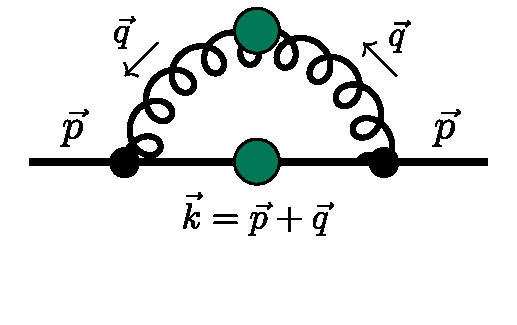
\includegraphics[scale=0.5, valign=c]{figures/quark_self_energy_classical_momenta} := \Sigma(p) &= (-ig)^2 T^{a}T^b \int \frac{\dd^4 q}{(2\pi)^4}\ \delta_{ab}\ \Pi^{\mu\nu}_{\bot}(q) G_A(q)\gamma_{\mu}G_q(p+q)\gamma_{\nu},
\end{align*}
with the transverse projection operator 
\begin{equation}
	\Pi^{\mu\nu}_{\bot}(p) = \delta^{\mu\nu} - \frac{p^{\mu}p^{\nu}}{p^2},
\end{equation}
and the spectral representations of the gluon propagator
\begin{align} 
G_A(p)&=\int_{0}^{\infty} \frac{\dd \lambda_A}{\pi} \frac{\lambda_A\rho_A(\lambda_A)}{p^{2}+\lambda_A^{2}},
\end{align}
and the quark propagator
\begin{equation}
	G_q(p^2) =  \slashed{p}\int\limits_0^\infty\frac{\dd\lambda}{\pi}\frac{\lambda\rho_1(\lambda)}{p^2+\lambda^2} + \int\limits_0^\infty\frac{\dd\lambda}{\pi}\frac{\lambda\rho_2(\lambda)}{p^2+\lambda^2}. \label{eqn:quarks}
\end{equation}
Note that the quark propagator is parametrized by two spectral functions, respecting the Dirac structure featuring a Dirac vector part $\sim \slashed{p}$ and a Dirac scalar part $\sim \mathbb{1}$, where the unit matrix has to be understood as the identity in Dirac space.\\
In a first step we split the diagram into its vector and scalar component:
\begin{equation}
	\Sigma_q(p^2) = \slashed{p}\cdot\Sigma_{\mathrm{vec}}(p^2) + \mathbb{1}\cdot\Sigma_{\mathrm{scal}}(p^2).
\end{equation}
Both terms involve two integrations, the usual loop momentum integration and the spectral integration. The integration order is swapped which is only allowed for the case of finite integrands due to Fubinis theorem. A schematic overview on how to renormalize and regularize the respective integrands properly, the spectral renormalization scheme, is presented above in Figure \ref{fig:spectral_renormalization}. The first task consists in manipulating the occurring tensor structures and momenta such that the momentum integrals can be evaluated analytically using standard formulas known in the context of dimensional regularization, i.\,e.
\begin{equation}
	\int\frac{\dd^d q}{(2\pi)^d}\frac{(q^2)^m}{\left[q^2 + \Delta\right]^n} = \frac{1}{(4\pi)^{d/2}}\frac{\Gamma(m+\frac{d}{2})\Gamma(n-\frac{d}{2}-m)}{\Gamma(\frac{d}{2})\Gamma(n)} \Delta^{m+d/2-m},
\end{equation} 
with $m$ a non-negative and $n$ a positive integer \cite{PeskinSchroeder1995}. For our computation the relevant expressions have $n=2$ and $m= 1,2$.
\begin{figure}[t]
\centering
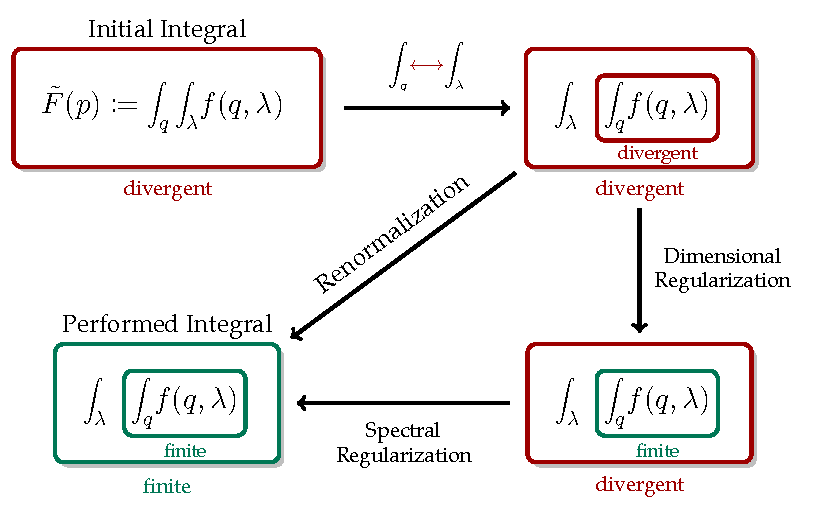
\includegraphics[width=0.8\textwidth]{figures/spectral_renormalization}
\caption[Applied regularization procedure.]{Applied regularization procedure. $f$ is some arbitrary divergent integrand. The two upper boxes have to be understood as finite by dimensional regularization but divergent in the limit $\varepsilon\rightarrow 0$. The first step consists of evaluating the momentum integral analytically using dimensional regularization before renormalizing the spectral integrands subsequently according to a BPHZ-renormalization scheme.}\label{fig:spectral_renormalization}
\end{figure}
The resulting expressions are evaluated in $d=4-2\varepsilon$ and expanded up to lowest order in $\varepsilon\rightarrow 0$. We are left with finite spectral integrands for $\varepsilon >0$, that in general need to be computed numerically. For numerical performance it is helpful to perform the spectral integrations at $\varepsilon=0$. The same is true for the access to the analytical momentum structure needed to extract the Minkowski properties. It is therefore required to set up a suitable renormalization procedure for the integrands in the limit $\varepsilon\rightarrow 0$. This means that it is not sufficient to discard the typical $\sim\frac{1}{\varepsilon}$-term after performing the momentum integrals to render the spectral integrands finite, which is a remnant of the swapping of the integration orders in the beginning. \\
The simplest way of regularizing the spectral integrands is by subtracting terms that render the expressions finite. This can be achieved for example by subtracting a Taylor series of the spectral integrand evaluated at the renormalization scale $\mu$ according to the BPHZ-scheme with Dyson's formula. \\
Note that the BPHZ-scheme in general does not preserve all symmetries of the theory at hand which is the same problem, that occurs when subtracting explicit counterterms in other schemes. The number of terms that need to be subtracted can be determined from naive power counting. Diagrammatically this can be visualized for our case as follows:
\begin{align*}
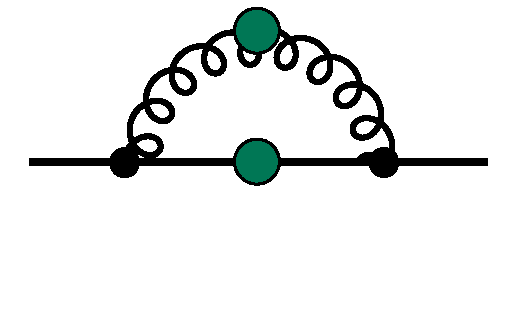
\includegraphics[scale=0.27, valign=c]{figures/quark_self_energy_classical} \longrightarrow 
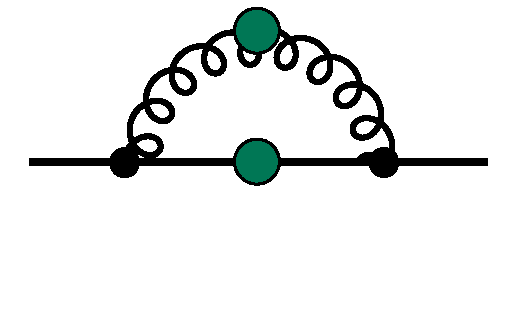
\includegraphics[scale=0.27, valign=c]{figures/quark_self_energy_classical} - \eval{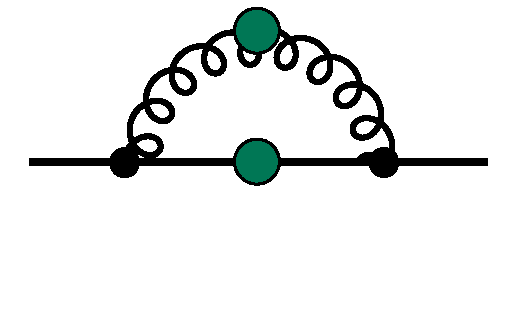
\includegraphics[scale=0.27, valign=c]{figures/quark_self_energy_classical}}_{p=\mu} -\ \frac{(p^2-\mu^2)}{2\mu}\left[\partial_{p}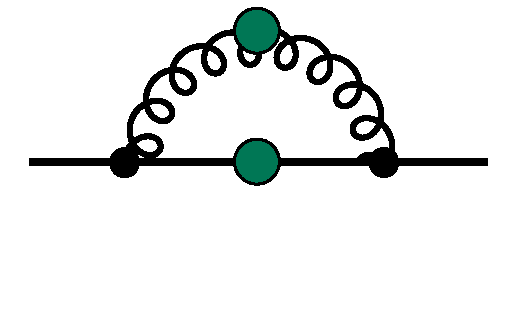
\includegraphics[scale=0.27, valign=c]{figures/quark_self_energy_classical}\right]_{p=\mu}
\end{align*}
The counterterms therefore explicitly contribute to the mass renormalization as well as to the wave function renormalization. They consistently remove the divergent parts of the integrands, we explicitly checked for UV-finiteness of all integrations. This finally allows us to solve the spectral integrals numerically after successfully performing the limit $\varepsilon\rightarrow 0$ beforehand. \\
The last step before being able to iteratively extract the spectral functions is the \enquote{analytic continuation} to Minkowski spacetime. This is achieved by replacing $p^0\rightarrow -i(\omega + i\varepsilon)$ and taking the limit $\varepsilon\rightarrow 0^+$. 
These integrands can now be used as our input for the numerical evaluation of the spectral integrals, after choosing suitable initial guesses for the spectral functions. More details on the numerical part of this work are presented in the subsequent section.\\
\section{A Few Words on Numerics}
The numerical part of the work is performed in Mathematica \cite{Mathematica}, since it provides all the tools to easily perform manipulations of the spectral integrands, the actual numerical integrations and the iterative procedure. \\

\noindent After computing the spectral integrands $\Sigma_{\mathrm{vec}}(p^2)$ and $\Sigma_{\mathrm{scal}}(p^2)$ and performing the respective spectral regularization as outlined above, we need to make initial guesses for the spectral densities to be able to perform the first iteration step. For the gluon spectral function (cf. Figure \ref{fig:gluon_specfunc}) we choose a result respecting the so called decoupling (or massive) solution for the gluon propagator in the infrared \cite{vonSmekalAlkoferHauck1997}. This may be adapted later to a solution respecting the known scaling scenario \cite{LercheVonSmekal2002}, which has been found to provide a dynamical generation of a mass gap for both the gluon and the ghost propagators, but is in general more complicated due to the non-trivial scaling exponent $\kappa$ with $\frac{1}{2}<\kappa < 1$. \\
For the initial quark spectral functions $\rho_1$ and $\rho_2$ we choose the respective \enquote{classical} spectral functions, i.\,e. the ones that reproduce the classical quark propagator:
\begin{figure}[t]
\hfill
\begin{subfigure}
	\centering
	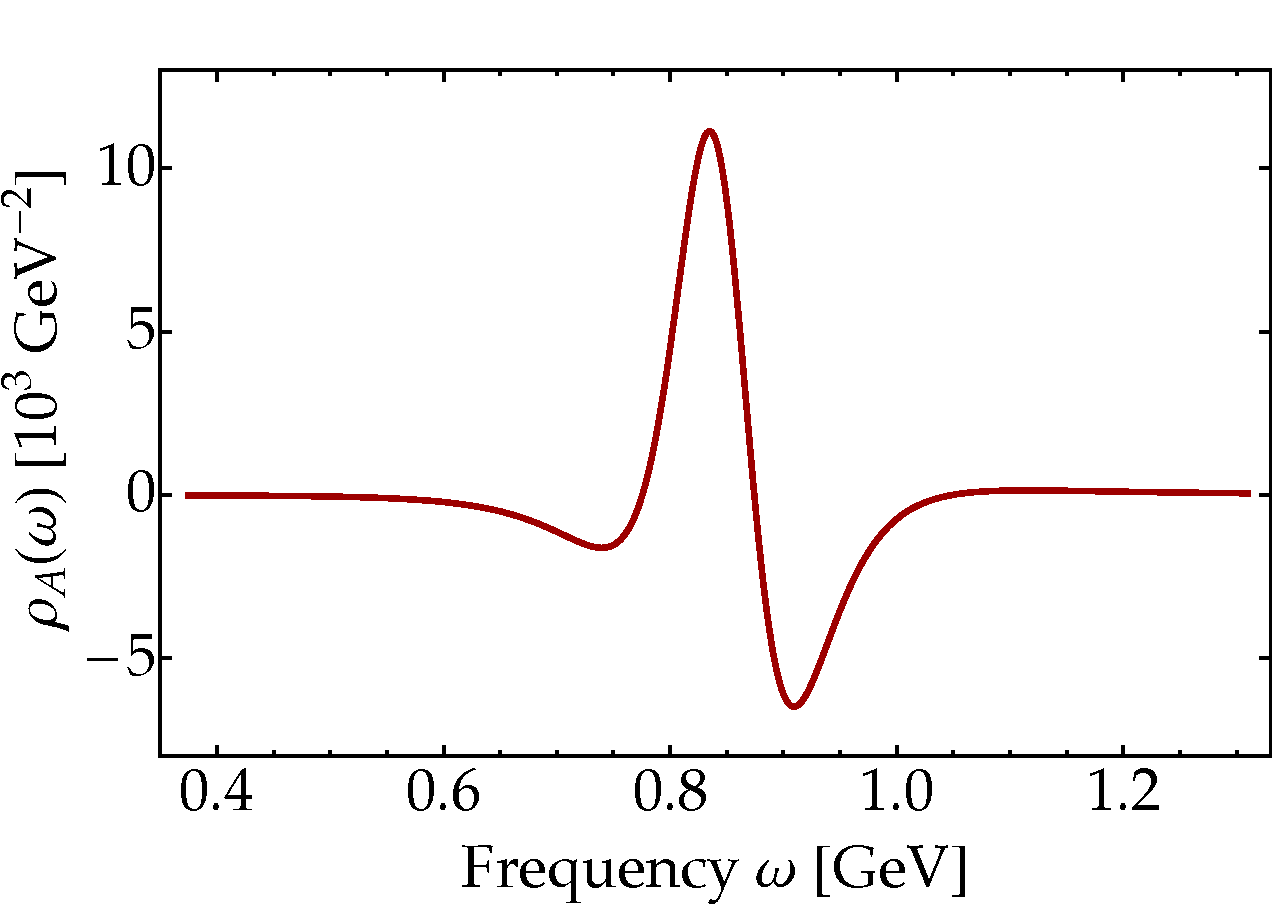
\includegraphics[width = 0.46\textwidth, trim= 4em 0 0 0]{figures/GluonSpecFuncPlot}
	%\subcaption{Gluon spectral function $\rho_A(\omega)$}
\end{subfigure}
\hfill
\begin{subfigure}
	\centering
	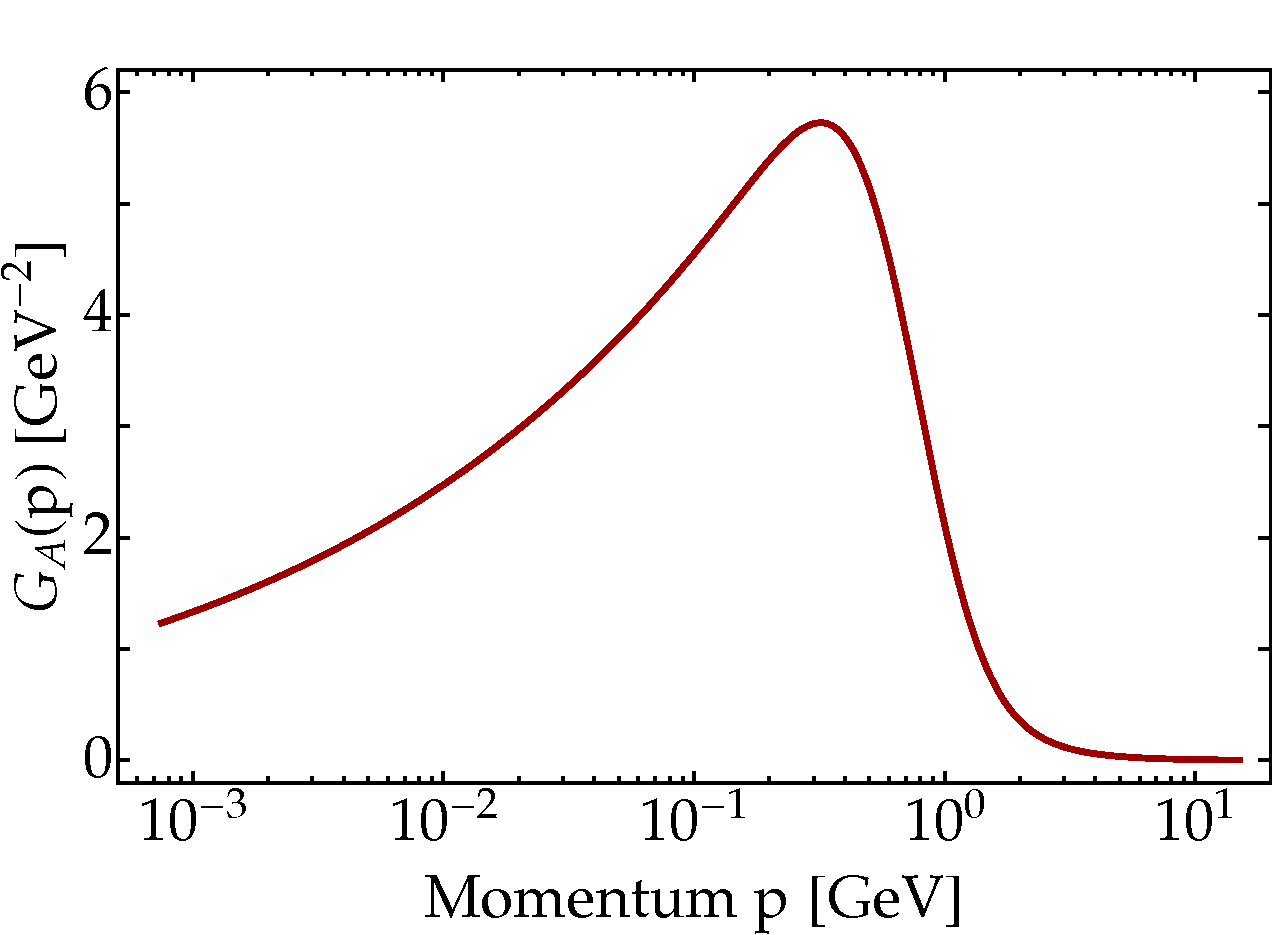
\includegraphics[width = 0.45\textwidth, trim= 4em 0 0 0]{figures/GluonPropPlot}
	\hfill
\end{subfigure}
	\caption{Chosen input gluon spectral function (left) and the corresponding propagator obtained from equation (\ref{eqn:KL_rep}) (right). This spectral function was computed by group members using the same techniques, results are not published yet.}
	\label{fig:gluon_specfunc}
\end{figure}


\begin{equation}
	\begin{aligned}
		\rho_{1,\mathrm{init}}(\lambda) &= 2\pi i\ \eval{\frac{\delta(\lambda-m_q)}{2\lambda}}_{\lambda=m_q}\\
		\rho_{2,\mathrm{init}}(\lambda) &= 2\pi m_q\ \eval{\frac{\delta(\lambda-m_q)}{2\lambda}}_{\lambda=m_q}.
	\end{aligned}
\end{equation}
As a final remark in this section we want to show how to explicitly extract the spectral functions $\rho_1$ and $\rho_2$ from the retarded quark propagator computed from the DSE. Schematically the inverse quark propagator is parametrized by two scalar dressing functions, i.\,e.
 \begin{equation}
 	G_q^{-1}(p^2) = i\slashed{p}\cdot A(p^2) + \mathbb{1}\cdot B(p^2)
 \end{equation}
 This leaves us with the following expression for the full propagator:
\begin{equation}
	G_q(p^2) = -i\slashed{p} \mathcal{A}(p^2; A,B) + \mathcal{B}(p^2; A,B) \equiv \slashed{p}\underbrace{\int\limits_0^\infty\frac{\dd\lambda}{\pi}\frac{\lambda\rho_1(\lambda)}{p^2+\lambda^2}}_{\equiv\ -i\mathcal{A}(p^2)} + \underbrace{\int\limits_0^\infty\frac{\dd\lambda}{\pi}\frac{\lambda\rho_2(\lambda)}{p^2+\lambda^2}}_{\equiv\ \mathcal{B}(p^2)}.
\end{equation}
Here we identified the respective parts of the propagator with the corresponding parts of the spectral representation (\ref{eqn:quarks}). \newpage
\begin{figure}[h]
	\centering
	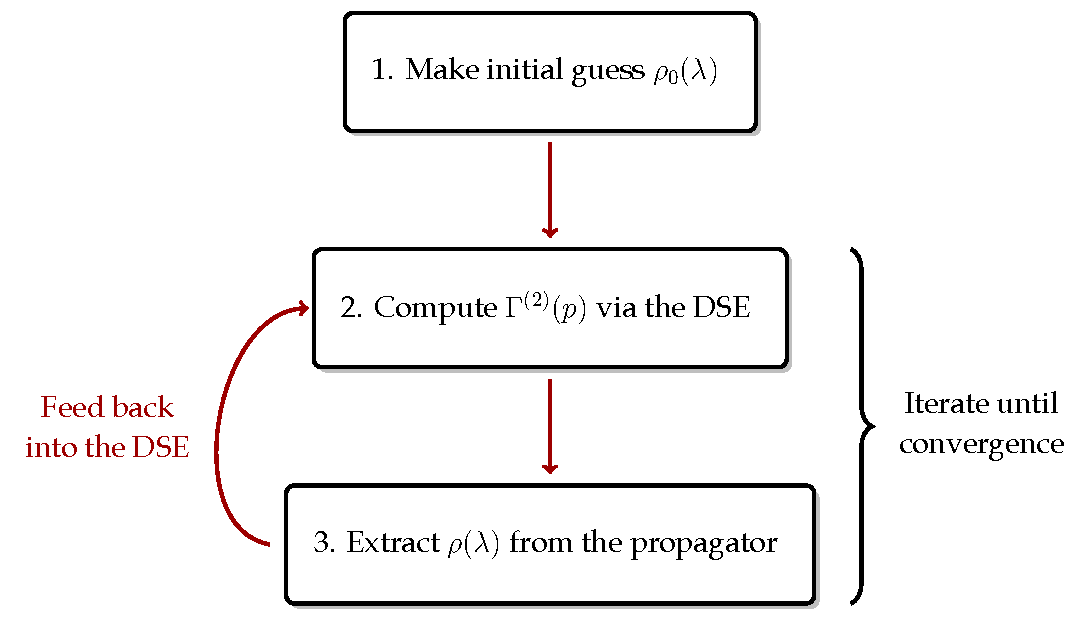
\includegraphics[width = 0.9\textwidth]{figures/iterative_computation}
	\caption{Iterative procedure to extract the spectral function from the inverse propagator obtained from the quark propagator DSE.} 
	\label{fig:code}
\end{figure}
\noindent The  scalar dressings here are related to $A(p^2)$ and $B(p^2)$ via
\begin{equation}
	\begin{aligned}
		\mathcal{A}(p^2) &= \frac{A(p^2)}{p^2A^2(p^2) + B^2(p^2)}, \\
		\mathcal{B}(p^2) &= \frac{B(p^2)}{p^2A^2(p^2) + B^2(p^2)}.
	\end{aligned}
\end{equation}
\noindent With this knowledge at hand, we use equation (\ref{eqn:specfunc_relation}) to find:

\begin{equation}
\begin{aligned}
	\rho_1(\omega) &= 2 \operatorname{Im}\left[\Pi_{\slashed{p}} G_{q}\left(-i(\omega + i0^+); \mathcal{A}, \mathcal{B}\right)\right] = 2 \operatorname{Im}\left[-i\mathcal{A}\left(-i(\omega + i0^+)\right)\right], \\
	\rho_2(\omega) &= 2 \operatorname{Im}\left[\Pi_{\mathbb{1}} G_{q}\left(-i(\omega + i0^+); \mathcal{A}, \mathcal{B}\right)\right]  = 2 \operatorname{Im}\left[\mathcal{B}\left(-i(\omega + i0^+)\right)\right],
\end{aligned}
\label{eqn:quark_specfuncs}
\end{equation}
with the projectors defined such that they allow us to access the relevant parts of the retarded propagator, i.\,e.
\begin{equation}
\begin{aligned}
	\Pi_{\slashed{p}}\left(\cdots\right) &= \operatorname{Tr}_{\mathrm{D}}\left[\frac{\slashed{p}}{p^2} \left(\cdots\right)\right],\\
	\Pi_{\mathbb{1}}\left(\cdots\right) &= \operatorname{Tr}_{\mathrm{D}}\left[\left(\cdots\right)\right].
\end{aligned}
\end{equation}
Here we used the fact that the trace of an odd number of gamma matrices vanishes. The index $\mathrm{D}$ refers to the Dirac trace.\\


\noindent With this initial setup at hand we can start the iteration and stepwise compute the spectral integrations, the Euclidean and real-time version of the scalar dressings of the inverse propagator $A(p^2/\omega^2)$ and $B(p^2/\omega^2)$ and of the full propagator $\mathcal{A}(p^2/\omega^2)$ and $\mathcal{B}(p^2/\omega^2)$ and finally extract the spectral functions for the quarks via equation (\ref{eqn:quark_specfuncs}). As an overview, the general structure of our code is visualized in Figure \ref{fig:code}. \\
A mandatory benchmark test for the correctness of the spectral function is of course the direct comparison of the Euclidean quark propagator with the the one obtained from the (updated) spectral function via equation (\ref{eqn:quarks}). 




